\chapter{字符串管理}

任何程序都需要管理字符串。管理就像分配、搜索、连接、扩展、收缩等等。

字符串需要许多操作。 尽管C标准库为这一目标提供了许多功能,但C经典字符串,即\code{char *}(或\code{char []})在PHP这样的强程序中按原样使用通常有点弱。

因此,PHP在C字符串之上设计了一个层:\keyword{zend\_strings}。另外还存在另一个API,它实现了C经典字符串或\keyword{zend\_strings}常见的字符串操作: \keyword{smart\_str} API。

\section{字符串管理:zend\_string}

它增加了内存管理功能,以便相同字符串可以在多个地方共享,而不需要复制它。另外一些字符串被“扣押”,即它们被“持久”分配并由内存管理器专门管理,因此它们不会在多个请求中被销毁。 这些内存稍后将从\href{http://www.phpinternalsbook.com/php7/memory_management/zend_memory_manager.html}{Zend内存管理器}获得永久分配。

\subsection{结构和访问宏}

下面是\keyword{zend\_string}结构:

\begin{lstlisting}[language=c]
struct _zend_string {
        zend_refcounted_h gc;           /*gc信息*/
        zend_ulong        h;            /* hash value */
        size_t            len;          /*字符串长度*/
        char              val[1];       /*字符串起始地址*/
};
\end{lstlisting}

如您所见,该结构嵌入了\code{zend\_refcounted\_h}头。这样做是为了内存管理和引用。由于字符串很可能用作哈希表查询的键,所以它将其哈希值嵌入到\keyword{h}字段中。这是一个无符号long \code{zend\_ulong}。
此数字仅在需要对\code{zend\_string}进行哈希处理时使用,尤其是与\href{http://www.phpinternalsbook.com/php7/internal_types/hashtables.html}{HashTables zend\_array}一起使用时; 这很可能。


如您所知,可以通过\keyword{len}字段知道字符串的长度,用来支持“二进制字符串”。二进制字符串是嵌入一个或多个\keyword{NUL}字符(\textbackslash{}0)的字符串。当传递给libc函数时,这些字符串将被截断,否则它们的长度将无法正确计算。所以在\keyword{zend\_string}中,字符串的长度总是已知的。请注意,计算ASCII字符(字节)数量的长度,不计算结尾的\keyword{NUL},但是计算可能在中间的NULs。例如,字符串“foo”在\keyword{zend\_string}中存储为“foo\textbackslash{}0”,其长度为3。此外,字符串“foo\textbackslash{}0bar”将存储为“foo\textbackslash{}0bar\textbackslash{}0”,长度将为7。

最后,字符存储在\code{char [1]}字段中。这不是一个\code{char *},而是一个\code{char[1]}。为什么?这是一种名为“C struct hack”的内存优化。(你可以搜索一下这些术语)。基本上,它允许引擎为\code{zend\_string}结构和要存储的字符分配空间,作为一个单独的C指针。这优化了内存访问,因为内存将是一个连续分配的块,而不是内存中稀疏的两个块
(一个用于\code{zend\_string *},一个用于存储到其中的\code{char *})。

struct hack一定要记住,因为内存布局看起来像C字符位于C \code{zend\_string}结构的末尾,在使用C调试器(或在调试字符串时)时可能会感觉到/看到。这个hack完全由你在操作\code{zend\_string}结构时使用的API管理。

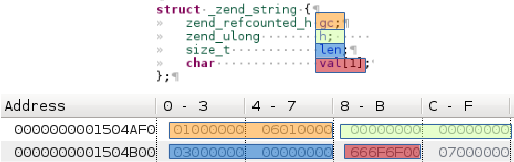
\includegraphics{images/zend_string_memory_layout.png} 

\subsection{使用\code{zend\_string}API}

\subsubsection{简单实例}

与\keyword{Zvals}一样,您不要手工操作\code{zend\_string}内部字段,而是始终要使用宏。还有一些宏可以触发字符串上的操作。这些不是函数,而是宏,都存储在所需的\href{https://github.com/php/php-src/blob/PHP-7.0/Zend/zend_string.h}{Zend/zend\_string.h }头:

\begin{lstlisting}[language=c]
zend_string *str;

str = zend_string_init("foo", strlen("foo"), 0);
php_printf("This is my string: %s\n", ZSTR_VAL(str));
php_printf("It is %zd char long\n", ZSTR_LEN(str));

zend_string_release(str);
\end{lstlisting}

上面的简单示例展示了基本的字符串管理。


